\documentclass[../main.tex]{subfiles}

\begin{document}
\section{Average temperature of each day of the year}
\subsection{Method}
The assignment is to take the average temperature of each day of each year. The analysis is started with a for loop over all the data points in the code. An if statement was then added in order to ignore all leap years, this was due to the short timescale of the project, and to simplify the task. For the years that is not a leap year the code goes into another if statement which checks if there have been several measurements on one day. The temperatures of one day is then summed up and divided with the number of temperatures for that day to receive the average. These average temperatures are then stored in one vector.

In order to sum up the temperature of one day for the different years two for loops were used. The first for loop goes through all the years and the second loop that is inside the first one loops over 365 days and adds each day into an array. This way the array will become the sum of the temperatures of one day for all the years. To receive the average another for loop were used that divided all elements of the array with the number of years.

To calculate the standard deviation, the formula for the standard deviation was used which can be seen in equation \ref{stdeq} below, where $\sigma$ denotes the standard deviation and $\mu$ is the mean.

\begin{equation}
\label{stdeq}
\sigma = \sqrt{\frac{1}{N} \sum ^N_{i=1} (x_i - \mu) }
\end{equation}
The code for the standard deviation can be seen in figure \ref{stdcode}. Two for loops were used one that loops over a full year (365 days). Inside that for loop another for loop was used to sum the standard deviation for the same day of each year.

\begin{figure}[H]
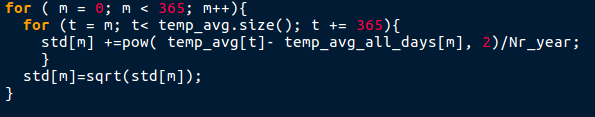
\includegraphics[scale= 0.5]{std_MNXB01.png}
\caption{The code for the standard deviation calculation, where temp$\_$avg is the average for all the days for all the years and temp$\_$all$\_$days is the average temperature of each day of the years. }
\label{stdcode}
\end{figure}
\subsection{Result and discussion}
The result which can be seen in figure \ref{avgtemp} shows the average temperature of each of the year for Lund.

\begin{figure}[H]
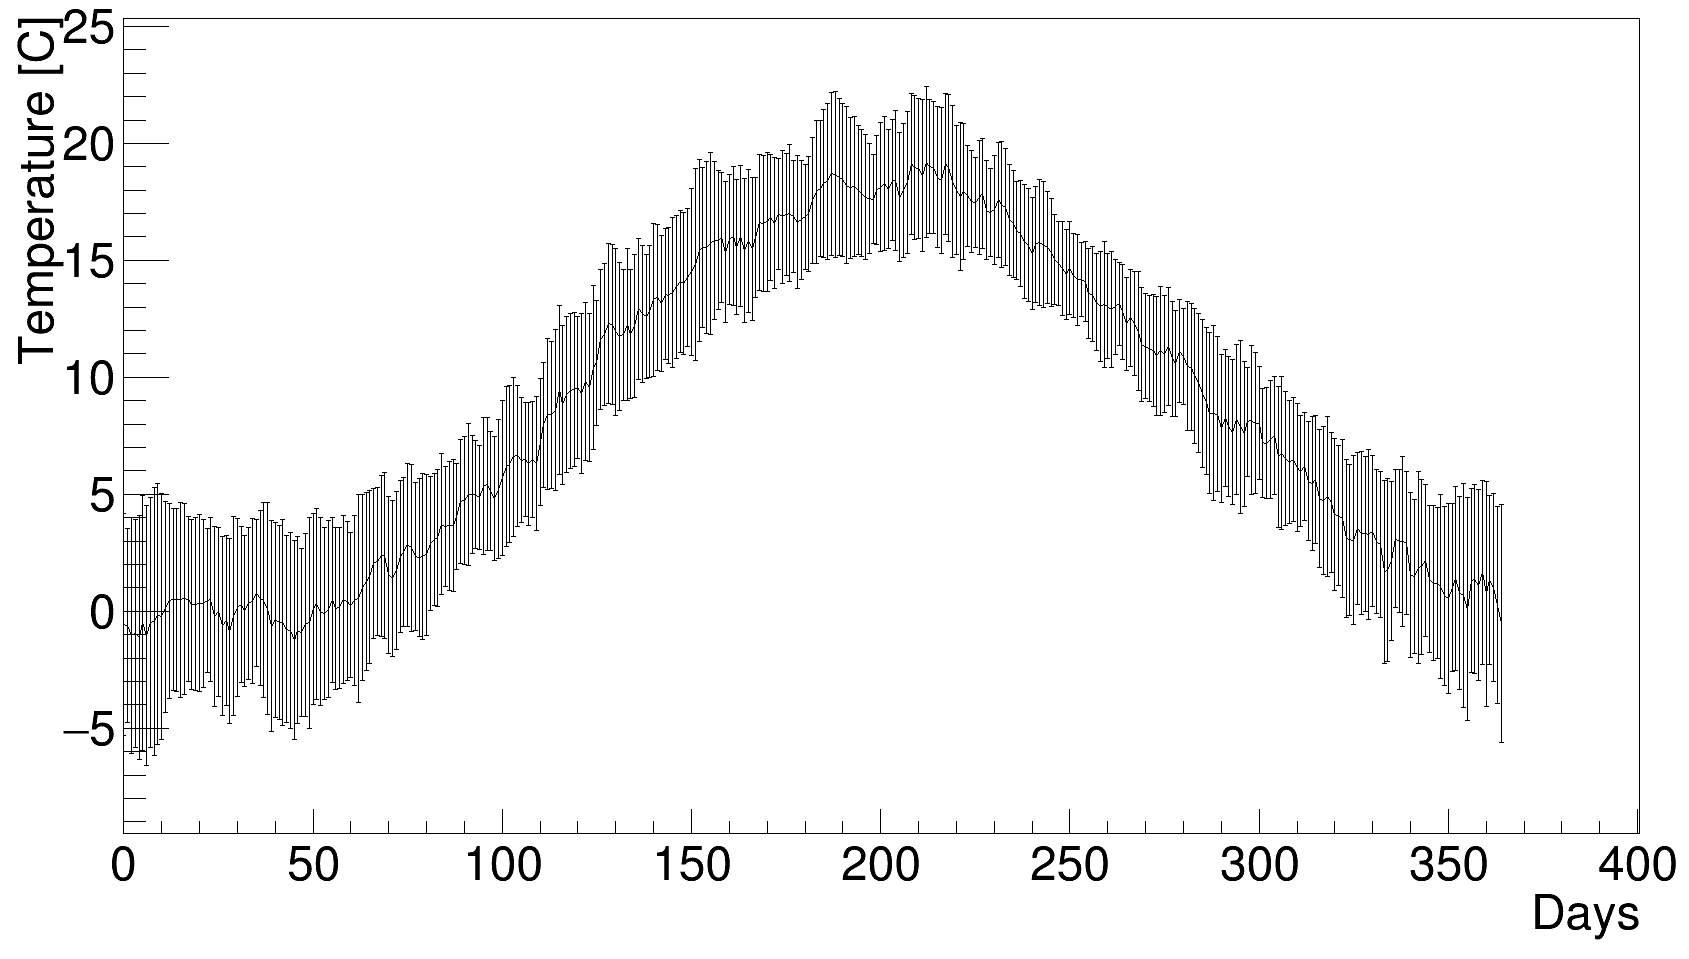
\includegraphics[scale = 0.2]{avg_temp.png}
\caption{The average temperature of each day of the year in Lund.}
\label{avgtemp}
\end{figure}


As can bee seen in figure \ref{avgtemp} the result is as one would expect, that the temperature is higher and more stable in the summer. In the winter it's colder and the temperature is less stable thus the larger standard deviation.

Even though the plot of the result gives an result that agrees with reality, the code has some major flaws. In order to simplify the task some assumptions were made which cost the accuracy of the result. One assumption that effected the result the most was the assumption that the dataset had measurements for all days which wasn't the case. The effect this have is that the days in the plot might not be at the right position in the plot thus not being accurate.

If we were to redo this task another approach would have been taken were the inconsistencies of the datasets would have been taken into account.



\end{document}